\documentclass[a4paper,11pt]{article} 
\usepackage[textwidth=17cm, top=0.4cm, bottom=1.4cm]{geometry} % для изменения размеров текста
\usepackage[english, russian]{babel} % для подключения русского языка 
\usepackage[unicode, pdftex]{hyperref} % для гиперссылок
\usepackage{color} % для измнения цвета гиперссылок
\usepackage[dvipsnames]{xcolor}
\usepackage{tabularx} % для таблиц 
\usepackage{multirow}
\usepackage[final]{graphicx} % для вставки картинок
\usepackage{framed} % обводка
\usepackage{amsmath} % матрицы

\hypersetup{
	colorlinks=true, % цветные ссылки
	linkcolor=blue, % цвет гиперссылок внутри документа
	urlcolor=blue % цвет ссылок на ресурсы в сети
}

\title{Blocks} 
\author{Виктор Пичугов}

\begin{document} 
	\maketitle
	\tableofcontents
	\newpage

	
	\section{Предисловие}
		В этом файлике я описываю примеры работы блоков, с которыми мне довелось поработать.
	
	\section{CFAR Detector}
	\subsection{Смысл блока CFAR Detector}
	Желательный свойством детектора является способность поддерживать заданную среднюю вероятность ложной тревоги $\overline{P}_{FA}$ в присутствии гетерогенных (неоднородных) или изменяющихся помех. Детектор, обладающий этим свойством, называется детектором с постоянной частотой ложных тревог. 
	
	Детекторы CFAR оценивают статистику помех $\widehat{g}_{Method}$, полученную в результате измерений радаром, и регулируют порог детектора $T_{Method}$ (threshold) для поддержания постоянной частоты ложных срабатываний или, что эквивалентно, $\overline{P}_{FA} = const$.
 	
 	\subsection{Архитектура CFAR Detector}
 	\begin{figure}[h!]
 		
 		\centering
 		
 		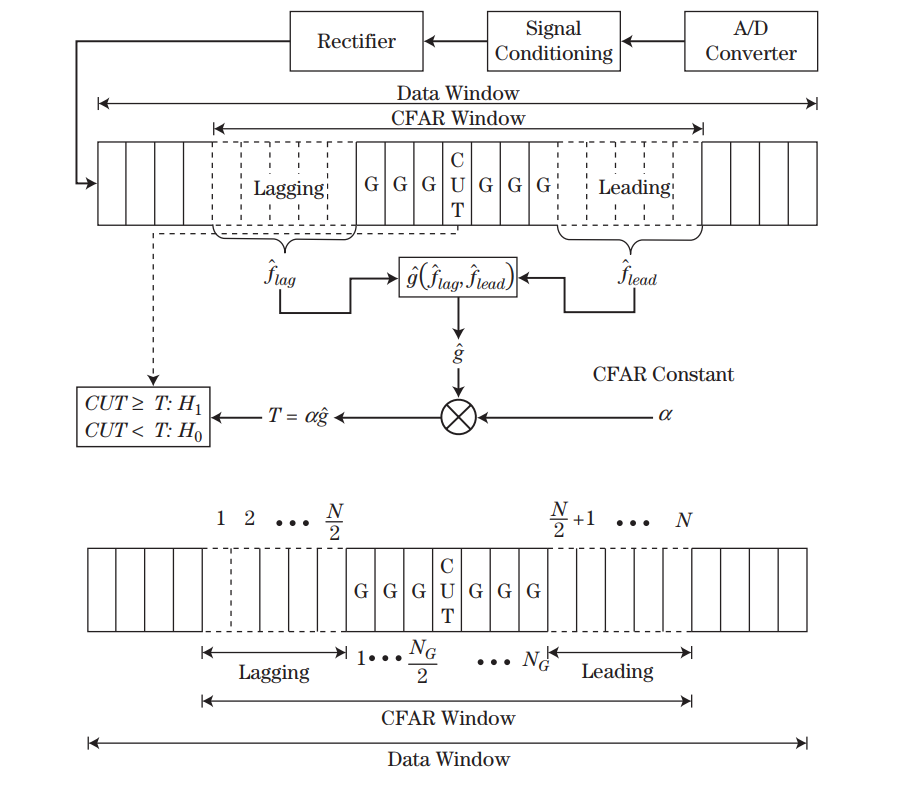
\includegraphics[width=0.6\linewidth]{Architecture.png}
 		
 		\caption{Архитектура блока CFAR Detector}
 		
 		%\label{fig:mpr}
 		
 	\end{figure}
 	
 	\subsection{Примечания}
 		Константа порогового значение $\alpha_{Method}$ вычисляется для белого Гауссовского шума.
 		
 		В настоящее время мы можем рассчитать порог $T_{Method}$ только тогда, когда на вход поступают одиночные импульсы (single pulses), без интегрирования импульсов.
 	
	\subsection{Примеры расчета порогового коэффициента, статистики помех}
		\subsubsection{CA - Cell Averaging}
			Пример 1. X - Vector(M,)
			Пусть:
			
			\begin{itemize}
				\item Number of guard cells - 0; (окружающие ячейки независимы)
				\item Number of training cells - 2;
				\item Threshold Factor Method - Auto;
				\item Probability of false alarm ($\overline{P}_{FA}$) - 0.1;
				\item Output Format - CUT result;
			\end{itemize}
			 
			$$X = [\colorbox{Cerulean}{5.825}, \colorbox{Apricot}{5.925}, \colorbox{Cerulean}{12.22}, 6.2, 2.525, 7.855, 1.725], Idx = 2$$
			
			Защитные ячейки не учавствуют в расчете, для вычисления оценки статистики $\widehat{g}_{CA}$, найдем среднее голубых ячеек:
			
			$$ \widehat{g}_{CA} = mean(z) = \frac{1}{2}\sum_{i = 1}^{2}z_{i} = \frac{5.825 + 12.22}{2} = 9.0225$$
			
			Для вычисления константы порогового значения $\alpha_{CA}$ воспользуемся формулой:
			
			$$ \alpha_{CA} = N \left[\overline{P}_{FA}^{-\frac{1}{N}} - 1\right] = 2 \left[0.1^{-0.5} - 1\right] = 4.324555320336758$$
			
			Порог $T_{Method}$ во всех методах в Matlab расчитывается по фомуле:
			
			$$ T_{Method} = \alpha_{Method}\cdot \widehat{g}_{Method} \Rightarrow $$
			
			$$ T_{CA} = \alpha_{CA}\cdot \widehat{g}_{CA} = 4.324555320336758 \cdot 9.0225 = 39.018300377738406$$
			
			\begin{framed}
				
			$$ T_{CA} = \colorbox{Apricot}{39.018300377738406}$$
			
			$$ \widehat{g}_{CA} = \colorbox{Apricot}{9.0225}$$ 
			
			$$ Y = [5.925 > 39.018300377738406] = \colorbox{Apricot}{[0]}$$
			\end{framed}
			
			Пример 2. X - Matrix(M, N)
			
			$$X = 
			\begin{bmatrix}
				\colorbox{Cerulean}{6.99} & \colorbox{Cerulean}{7.09} & \colorbox{Cerulean}{6.354}\\
				\colorbox{Apricot}{13.38} & \colorbox{Apricot}{7.365} & \colorbox{Apricot}{4.19}\\
				\colorbox{Cerulean}{3.69} & \colorbox{Cerulean}{9.02} &	 \colorbox{Cerulean}{8.33}\\
				2.89 & 7.855 & -2.79
			\end{bmatrix}, Idx = 2
			$$
			
			$$ \widehat{g}_{CA} = \left[\frac{6.99 + 3.69}{2}, \frac{7.09 + 9.02}{2}, \frac{6.354 + 8.33}{2}\right] = [5.34,  8.055,  7.342]$$
			
			$$ \alpha_{CA} = N \left[\overline{P}_{FA}^{-\frac{1}{N}} - 1\right] = 2 \left[0.1^{-0.5} - 1\right] = 4.324555320336758$$
			
			$$ T_{CA} = \alpha_{CA}\cdot \widehat{g}_{CA} = broadcast(*, \alpha_{CA}, \widehat{g}_{CA})= [23.0931,  34.8343,  31.7509] $$
			
			\begin{framed}
				
				$$ T_{CA} =  \colorbox{Apricot}{[23.0931,  34.8343,  31.7509]}$$
				
				$$ \widehat{g}_{CA} =  \colorbox{Apricot}{[5.34,  8.055,  7.342]}$$ 
				
				$$ Y = [13.38 > 23.0931, 7.365 > 34.8343, 4.19 > 31.7509] = \colorbox{Apricot}{[0, 0, 0]}$$
			\end{framed}
		
		\subsubsection{GO - Greatest of Cell Averaging}
			Пример 1. X - Vector(M,)
			Пусть:
			
			\begin{itemize}
				\item Number of guard cells - 4; 
				\item Number of training cells - 4;
				\item Threshold Factor Method - Auto;
				\item Probability of false alarm ($\overline{P}_{FA}$) - 0.1;
				\item Output Format - CUT result;
			\end{itemize}
			
			$$X = 
			\begin{bmatrix}
				1.421\\
				2.12\\
				1.169\\
				\colorbox{Cerulean}{1.607}\\
				\colorbox{Cerulean}{1.235}\\
				\colorbox{LimeGreen}{1.214}\\
				\colorbox{LimeGreen}{1.641}\\
				\colorbox{Apricot}{1.232}\\
				\colorbox{LimeGreen}{2.067}\\
				\colorbox{LimeGreen}{1.46}\\
				\colorbox{Cerulean}{1.357}\\
				\colorbox{Cerulean}{1.519}\\
				1.332\\
				1.357\\
				1.534
			\end{bmatrix}, Idx = 8
			$$
			
			$$ \widehat{g}_{GO} = \max(mean(\widehat{f}_{GO,lag}), mean(\widehat{f}_{GO,lead})) = \max(\widehat{f}_{GO,lag}, \widehat{f}_{GO,lead}) = \max\left(\frac{1}{\frac{N}{2}}\sum_{i = 1}^{\frac{N}{2}}z_{i},\frac{1}{\frac{N}{2}}\sum_{i = \frac{N}{2} + 1}^{N}z_{i}\right)$$
			
			$$ \widehat{f}_{GO,lag} = \frac{1.607 + 1.235}{2} = 1.421$$ 
			$$ \widehat{f}_{GO,lead} = \frac{1.357 + 1.519}{2} = 1.438$$ 
			$$ \widehat{g}_{GO} = \max(1.421, 1.438) = 1.438 $$
			
			$$ CAThreshold = N \left[\overline{P}_{FA}^{-\frac{1}{N}} - 1\right] = 4 \left[0.1^{-0.25} - 1\right] = 3.113117640155691$$
			
			$$ \alpha_{GO} = |fzero(4, 0.1, |CAThreshold|, Rank=1)| = 2.341796132759153$$ 
			
			$$ T_{GO} = \alpha_{GO}\cdot \widehat{g}_{GO} = 2.341796132759153 \cdot 1.438 = 3.367502838907662$$
			
			\begin{framed}
				
				$$ T_{GO} =  \colorbox{Apricot}{3.367502838907662}$$
				
				$$ \widehat{g}_{GO} =  \colorbox{Apricot}{1.438}$$ 
				
				$$ Y = [1.232 > 3.367502838907662] = \colorbox{Apricot}{[0]}$$
			\end{framed}
			
			
		\subsubsection{SO - Smallest of Cell Averaging}
			Пример 1. X - Vector(M,)
			
			\begin{itemize}
				\item Number of guard cells - 4; 
				\item Number of training cells - 4;
				\item Threshold Factor Method - Auto;
				\item Probability of false alarm ($\overline{P}_{FA}$) - 0.1;
				\item Output Format - CUT result;
			\end{itemize}
			
			$$X = 
			\begin{bmatrix}
				1.421\\
				2.12\\
				1.169\\
				1.607\\
				\colorbox{Cerulean}{1.235}\\
				\colorbox{Cerulean}{1.214}\\
				\colorbox{LimeGreen}{1.641}\\
				\colorbox{LimeGreen}{1.232}\\
				\colorbox{Apricot}{2.067}\\
				\colorbox{LimeGreen}{1.46}\\
				\colorbox{LimeGreen}{1.357}\\
				\colorbox{Cerulean}{1.519}\\
				\colorbox{Cerulean}{1.332}\\
				1.357\\
				1.534
			\end{bmatrix}, Idx = 9
			$$
			
			$$ \widehat{g}_{SO} = \min(mean(\widehat{f}_{SO,lag}), mean(\widehat{f}_{SO,lead})) =\min(\widehat{f}_{SO,lag}, \widehat{f}_{SO,lead}) = \min\left(\frac{1}{\frac{N}{2}}\sum_{i = 1}^{\frac{N}{2}}z_{i},\frac{1}{\frac{N}{2}}\sum_{i = \frac{N}{2} + 1}^{N}z_{i}\right)$$
			
			$$ \widehat{f}_{SO,lag} = \frac{1.607 + 1.235}{2} = 1.2245$$ 
			$$ \widehat{f}_{SO,lead} = \frac{1.357 + 1.519}{2} = 1.4255$$ 
			$$ \widehat{g}_{SO} = \min(1.2245, 1.4381.4255) = 1.2245$$
			
			$$ CAThreshold = N \left[\overline{P}_{FA}^{-\frac{1}{N}} - 1\right] = 4 \left[0.1^{-0.25} - 1\right] = 3.113117640155691$$
			
			$$ \alpha_{SO} = |fzero(4, 0.1, |CAThreshold|, Rank=1)| = 6.509460338847331$$
			
			$$ T_{SO} = \alpha_{SO}\cdot \widehat{g}_{SO} = 6.509460338847331 \cdot 1.2245 = 7.970834184918557$$
			
			\begin{framed}
				
				$$ T_{SO} =  \colorbox{Apricot}{7.970834184918557}$$
				
				$$ \widehat{g}_{GO} =  \colorbox{Apricot}{1.2245}$$ 
				
				$$ Y = [2.067 > 7.970834184918557] = \colorbox{Apricot}{0}$$
			\end{framed}
			
		\subsubsection{OS - Order Statistics}
			Пример 1. X - Vector(M,)
		
			\begin{itemize}
				\item Rank 2;
				\item Number of guard cells - 4; 
				\item Number of training cells - 4;
				\item Threshold Factor Method - Auto;
				\item Probability of false alarm ($\overline{P}_{FA}$) - 0.1;
				\item Output Format - CUT result;
			\end{itemize}
			
			$$X = 
			\begin{bmatrix}
				1.421\\
				2.12\\
				1.169\\
				1.607\\
				\colorbox{Cerulean}{1.235}\\
				\colorbox{Cerulean}{1.214}\\
				\colorbox{LimeGreen}{1.641}\\
				\colorbox{LimeGreen}{1.232}\\
				\colorbox{Apricot}{2.067}\\
				\colorbox{LimeGreen}{1.46}\\
				\colorbox{LimeGreen}{1.357}\\
				\colorbox{Cerulean}{1.519}\\
				\colorbox{Cerulean}{1.332}\\
				1.357\\
				1.534
			\end{bmatrix}, Idx = 9
			$$
			
			$$ \widehat{g}_{OS} = sort(X) = 
			sort\begin{bmatrix}
				\colorbox{Cerulean}{1.235}\\
				\colorbox{Cerulean}{1.214}\\
				\colorbox{Cerulean}{1.519}\\
				\colorbox{Cerulean}{1.332}
			\end{bmatrix} = 
			\begin{bmatrix}
				\colorbox{Cerulean}{1.214}\\
				\colorbox{Cerulean}{1.235}\\
				\colorbox{Cerulean}{1.332}\\
				\colorbox{Cerulean}{1.519}
			\end{bmatrix}
			, sort(X)[Rank] = sort(X)[2] = 1.235
			$$
			
			$$ T_{OS} = \alpha_{OS} \cdot \widehat{g}_{OS}$$
		
			$$ CAThreshold = N \left[\overline{P}_{FA}^{-\frac{1}{N}} - 1\right] = 4 \left[0.1^{-0.25} - 1\right] = 3.113117640155691$$
			$$  \alpha_{OS} = fzero(4, 0.1, CAThreshold, Rank=2) = 7.4688259109311740890688259109312 $$
			$$ T_{OS} = 7.4688259109311740890688259109312 * 1.235 = 9.224 $$
			
			\begin{framed}
				
				$$ T_{OS} =  \colorbox{Apricot}{9.224}$$
				
				$$ \widehat{g}_{OS} =  \colorbox{Apricot}{1.235}$$ 
				
				$$ Y = [2.067 > 9.224] = \colorbox{Apricot}{0}$$
			\end{framed}
		
	
			\noindent\rule{\textwidth}{2pt} 
	

	\section{CFAR Detector 2D}	

		По сути, CFAR Detector 2D работает также, как и одномерный. Сейчас покажу в чем различия.
		
		\subsection{CA - Cell Averaging}
		Пример 1. X - Matrix(M, N, K)
		
		\begin{itemize}
			\item GuardBandSize - 0; 
			\item NumTrainingCells - [2, 1];
			\item Threshold Factor Method - Auto;
			\item Probability of false alarm ($\overline{P}_{FA}$) - 0.1;
			\item Output Format - CUT result;
		\end{itemize}
		
		$$
		Idx = 
		\begin{bmatrix}
			3 & 3 & 3 & 3\\
			2 & 3 & 4 & 5
		\end{bmatrix}
		$$
		Вот тут надо по-медленее. У нас в распоряжении 4 элемента: $[3, 2], [3, 3], [3, 4], [3, 5]$. Теперь для каждого элемента из $Idx$ для каждой матрицы $X[:, :, i]$ рассчитывается статистики $\widehat{g}_{Method}$. Например, для элемента $[3, 2]$ получается такая картина. Не забываем, что область расчета для каждой ячейки $[1, 2]$.
		
		$$X[:, :, 1] = 
		\begin{bmatrix}
			 \colorbox{Cerulean}{0.3405} & \colorbox{Cerulean}{0.4562} & \colorbox{Cerulean}{0.5847} & 0.8753 & 0.9131 & 0.3587\\
			 \colorbox{Cerulean}{0.3703} & \colorbox{Cerulean}{0.6264} & \colorbox{Cerulean}{0.5992} & 0.6108 & 0.8785 & 0.8746\\
			 \colorbox{Cerulean}{0.0927} & \colorbox{Apricot}{0.3006} & \colorbox{Cerulean}{0.9646} & 0.2729 & 0.081 & 0.9238\\
			 \colorbox{Cerulean}{0.5937} & \colorbox{Cerulean}{0.5477} & \colorbox{Cerulean}{0.7804} & 0.9249 & 0.7785 & 0.066\\
			 \colorbox{Cerulean}{0.9422} & \colorbox{Cerulean}{0.7789} & \colorbox{Cerulean}{0.4621} & 0.6751 & 0.9459 & 0.0758\\
			 0.9737 & 0.7881 & 0.4712 & 0.6059 & 0.1029 & 0.8549
		\end{bmatrix},$$
		$$ 
		X[:, :, 2] = 
		\begin{bmatrix}
			 \colorbox{Cerulean}{0.9488} & \colorbox{Cerulean}{0.8312} & \colorbox{Cerulean}{0.833} & 0.902 & 0.0536 & 0.152\\
		     \colorbox{Cerulean}{0.4265} & \colorbox{Cerulean}{0.6524} & \colorbox{Cerulean}{0.399} & 0.3634 & 0.5333 & 0.3657\\
			 \colorbox{Cerulean}{0.1149} & \colorbox{Apricot}{0.4204} & \colorbox{Cerulean}{0.5529} & 0.604 &  0.9317 & 0.7697\\
			 \colorbox{Cerulean}{0.4929} & \colorbox{Cerulean}{0.0506} & \colorbox{Cerulean}{0.5763} & 0.3867 & 0.684 & 0.4179\\
			 \colorbox{Cerulean}{0.8446} & \colorbox{Cerulean}{0.6383} & \colorbox{Cerulean}{0.6795} & 0.5688 & 0.1191 & 0.3555\\
			 0.2888 & 0.9298 & 0.7851 & 0.7652 & 0.0636 & 0.0592
		\end{bmatrix}
		$$
		
		$$ \widehat{g}_{CA} = mean(X) = 
		mean\begin{bmatrix}
		 	\colorbox{Cerulean}{0.3405} & \colorbox{Cerulean}{0.4562} & \colorbox{Cerulean}{0.5847}\\
			\colorbox{Cerulean}{0.3703} & \colorbox{Cerulean}{0.6264} & \colorbox{Cerulean}{0.5992}\\
			\colorbox{Cerulean}{0.0927} & & \colorbox{Cerulean}{0.9646}\\
			\colorbox{Cerulean}{0.5937} & \colorbox{Cerulean}{0.5477} & \colorbox{Cerulean}{0.7804}\\
			\colorbox{Cerulean}{0.9422} & \colorbox{Cerulean}{0.7789} & \colorbox{Cerulean}{0.4621}\\
		\end{bmatrix} = 0.5814
		$$
		
		$$ T_{CA} = \alpha_{CA} \cdot \widehat{g}_{CA}$$
		$$  \alpha_{CA} = 2.502760887110222 $$
		$$ T_{CA} = 0.5814 \cdot 2.502760887110222 = 1.4551051797658832$$
	
		По аналогии остается рассчитать статистики для остальные элементов. Итого у нас получится матричка $[4, 2]$. Тоесть $4$ - это вторая размерность $Idx$ и $2$ это 3 размерность матрицы $X$. 
		
		\begin{framed}
			
			$$ T_{CA} =  \colorbox{Apricot}{1.4551051797658832}$$
			
			$$ \widehat{g}_{CA} =  \colorbox{Apricot}{0.5814}$$ 
			
			$$ Y = [0.3006 > 1.4551051797658832] = \colorbox{Apricot}{0}$$
		\end{framed}
	
		
		
	\noindent\rule{\textwidth}{2pt} 

	\section{MVDR Spectrum}
	
	\noindent\rule{\textwidth}{2pt} 
	\section{Beamscan Spectrum}
	\noindent\rule{\textwidth}{2pt} 
	
	\section{Propagation delay}
	\noindent\rule{\textwidth}{2pt} 
	
\end{document} 

